% tex file for convolution
\subsubsection{Convolution}
\par \indent Our study is structured around event-related neurological 
stimulus, not block stimulus as was discussed as the in-class example. We 
predicted the hemoglobin response (HR) related to this type of neurological 
stimulus, since the methods in class were much better for block stimulus. 

We approached the problem multiple ways, trying to better replicate the 
predicted response function defined by:

\begin{equation} \label{eq:convolve}
r(t)= \sum_{i=1}^n \psi_{i} \phi_{i}(t-t_i)
\end{equation}

where $\psi$ is the amplitude of the response stimulis (always $1$ in our case),
 and $\phi_{i}$ is the hemodyamic response started at the $i$th  stimulation 
 ($t_i$).

The 5 approaches could be catorgories into 3 subcategory \textbf{(1)} a strict replication of \ref{eq:convolve}, \textbf{(2)} a similar function as (1) that 
utilizes matrix multiplication, \textbf{(3)} a function that slit the intervals 
between each scan (2 seconds) into a certain number of even slices, then put 
the stimulus into the closed split, used \texttt{np.convolve} on this stimulus 
and a detailed hrf function, and then reduce the output back into the 2 second 
time intervals. Detailed exploration of this matter can be found in the 
appendix.

We compared these methods based on accuracy and speed. Selecting a model similar
to the subcategory (3), with 15 slices between each 2 second scan capture. Figure
\ref{fig:convolution} displaces accuracy comparison, and table 
\ref{table:convolution} show the accuracy based off of \texttt{ipython}'s 
\texttt{timeit} function.



\begin{figure}[ht]
\centering
	\begin{minipage}[b]{0.45\linewidth}
		\centering
		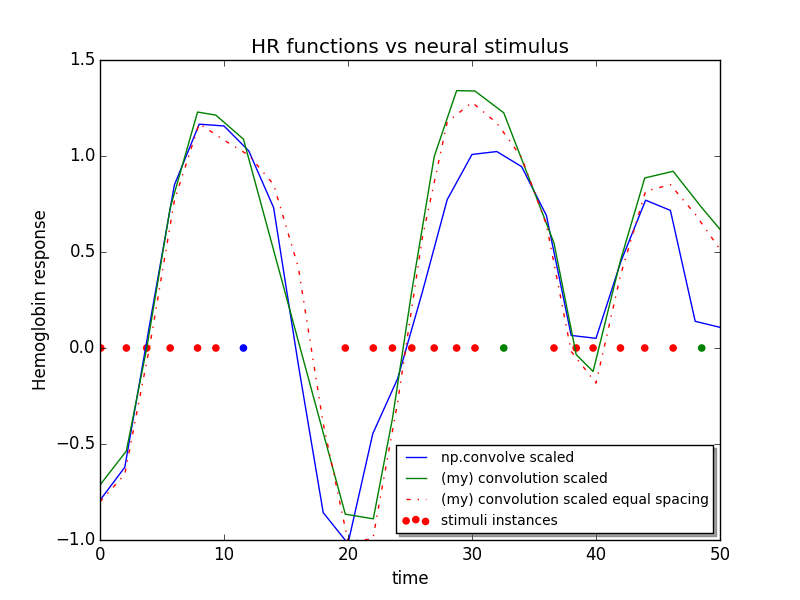
\includegraphics[width=.8\linewidth]{images/convolution_vs_neural_stimulus}  
		% needs to be from the event_related_HRF_script2.py 
		\caption{\scriptsize{Different convolution functions vs the Nueral stimulus}}
		\label{fig:convolution}

	\end{minipage}
\quad
	\begin{minipage}[b]{0.45\linewidth}
		\centering
		\begin{tabular}{|l | c|}
		\hline
		name in graph & Speed per loop \\
		\hline
		np    			 & 14.4 µs \\
		user 2     		 & 972 ms  \\
		user 3     		 & 1.15 s  \\
		user 4 (15 cuts) & 98.3 ms \\
		user 4 (30 cuts) & 185 ms  \\
		user 5     	 	 & 110 ms  \\
		\hline
		\end{tabular}
		\vspace{5mm}
		\caption{\scriptsize{Speed to create HRF predictions for Subject 001, all conditions}}
		\label{table:convolution}
	\end{minipage}
\end{figure}

The "np" run is the worst, and extremely theoretically incorrect (and the whole reason we did the rest of the analysis). The "user 2" and "user 3" fall under the first subcategory and  "user 5" falls under the 2nd subcategory, and "user 4" fall under the 3rd subcategory, with notations for the number of slices between each scan.



\subsubsection{Time Correction}

Since the fMRI machine actually scans each voxel at a slightly different time (in our case the lowest horizontal slice was scanned first, and it worked up toward the top of the brain), there was observable drift, which needed to be accounted for.

We did so by shifting the times of stimulus "backwards" for voxels scanned later, and to directly "correct" for the delay of the scan (assuming that each layer of the scan took 2/34 of a second).

\subsubsection{Multiple Conditions}
At the beginning of our analysis we tried to see if there was strength in 
seperating our 3 conditions and creating seperate predicted hemodyamic reponses 
for each (to allow for different applitudes for each type of condition), at 
that time it didn't seem to be very different in the $\beta$ values we got, so 
we didn't continue the exploration. It is quiet possible that with the new 
approaches we've applied in the overall paper, that exploration into the 
differentiating the conditions for the stimulus might see gains in 
interpretability.


